\newpage

\section{فصل سوم}

در فصل یک و دو در مورد قدم اول  مهندسی نیازمندی یعنی جمع‌آوری اطلاعات صحبت شد.
در این فصل در مورد بررسی و ارزیابی داده‌های جمع‌آوری شده مرحله قبل صحبت خواهیم
کرد. نتیجه‌ای که این مرحله دارد آن است که همه اعضای تیم به یک اجماع و توافق بر
سر تمام مواردی که انتخاب شده است برسند.

\subsection{چهار کار اصلی ارزیابی داده‌های جمع‌آوری شده}

\begin{enumerate}
    \item \lr{Inconsistency management}: مدیریت ناسازگاری, نویسنده کتاب در شرایط
    خاصی که دو چیز با هم سازگاری ندارند را می‌گوید ناسازگار است و گاهی در برخی
    قسمت‌های کتاب از کلمه تضاد یا \lr{Conflict} استفاده کرده است. تضاد زمانی رخ
    می‌دهد که جملات با هم تضاد داشته باشد. \begin{enumerate}
        \item اگر بین جملات تناقص باشد به آن می‌گویند تضاد یا \lr{Conflict} که
        در نیازمندی‌های نرم‌افزاری، نیازمندی سیستم و \lr{Assumption}ها رخ
        می‌دهد.
        \item اگر تناقص بین المان‌ها باشد می‌گویند المان‌ها ناسازگاری دارند.
    \end{enumerate}
    \item \lr{Risk analysis}: بررسی ریسک‌ها \begin{enumerate}
        \item در حقیقت تمام اتفاقاتی را می‌گوید که ممکن است در برابر آنها
        کارهایی انجام بدهیم یا قابلیتی را طراحی کنیم که معمولاً محیطی،
        نرم‌افزاری و دامنه‌ای هستند.
        \item برای مثال: فراموشی گذرواژه یک بررسی ریسک بوده است، که پیامک شدن
        گذرواژه یا \lr{OTP} به صورت عامل محیطی یا \lr{Assumption} بوده، طراحی
        لاگین و فرم فراموشی گذرواژه از نوع نیازمندی نرم‌افزاری که در برابر ریسک
        تمهیداتی در نظر گرفته شده است.
        \item نکته مهم در ریسک‌ها آن است که هیچ وقت در زمان جمع‌آوری داده‌ها
        ریسک را بررسی نمی‌کنیم چون ممکن است ناخودآگاه برخی موارد را ریسک در نظر
        بگیریم و در جمع‌آوری آنها حساس شویم.
        \item می‌تواند در خصوص مجموعه اقداماتی باشد که در سیستم تکرار پذیر‌اند
        مانند تحلیل‌گر ریسک در سیستم‌های مخشص مانند سیستم‌های مالی
        \item ریسک \lr{Not} یک جمله می‌باشد.
        \item ریسک برای یک جمله می‌باشد، اما تضاد‌ها برای دو یا چند جمله می‌باشد
        (به تمرین \lr{p2.pdf} مراجعه شود).
    \end{enumerate}
    \item انتخاب بین گزینه‌ها: بعد از ریسک‌ها گزینه‌هایی که به نظرم مناسب بوده
    است که فیلتر کردیم را بایستی بین آنها یکی را انتخاب کنیم که در سیستم نهایی
    خود استفاده کنیم.
    \item اولویت‌بندی کردن کار‌ها: همه کار‌ها در یک سطح اهمیت نخواهند بود. پس
    نیازمند اولویت‌بندی کار‌های مشخص شده در مرحله قبل هستیم. یکی از بارزترین
    مثال‌ها نسخه‌بندی کردن کار‌ها می‌باشد.
\end{enumerate}

\subsection{ناسازگاری‌ها}

ناسازگاری بین المان‌های دانشی اتفاق می‌افتد که مرتبه تکرار بسیار زیادی در مهندسی
نیازمندی دارد. معمولا دو بُعد ناسازگاری وجود دارد:

\begin{itemize}
    \item \lr{Inter-viewpoint}: مربوط به \lr{NFR}ها نیست و معمولاً ذینفعان تمرکز
    و نگرانی‌های خودشان را دارند. برا مثال کارشناس دامنه در برابر بخش بازاریابی.
    \item \lr{Intra-viewpoint}: خواسته‌های مختلف کاربران که به صورت عملیاتی
    هستند. حلشان با استفاده از الگوریتم‌ها امکان‌پذیر می‌باشد.
\end{itemize}

ناسازگاری‌ها به ۳ دسته تقسیم می‌شوند تا قبل از طراحی توسط طراح سیستم همه با این
مفاهیم به اجماع برسند:

\subsubsection{تصادم معنایی یا \lr{Terminology clash}}

استفاده از چندین نام برای یک مفهوم مشترک را می‌گوید.

\begin{itemize}
    \item کسی در دانشگاه درس می‌دهد نام‌های مختلفی دارد: استاد، دکتر، مدرس
    \item کسی که کتاب را از کتابخانه قرض می‌گیرد: کاربر، قرض‌گیرنده، متشری یا
    \lr{Patron}
\end{itemize}

این تضاد معنایی به گونه‌ای است که هر معنا یک کلاس خاص خواهد بود که هیچ ربطی
ندارند تا به یکدگیر متصل شوند.

\subsubsection{تصادم در تعیین و طراحی یا \lr{Designation clash}}

استفاده از یک نام برای چند مفهوم مختلف را می‌گوید.
برای مثال: کسانی که در دانشگاه کار می‌کنند را کارمند می‌گویند. این کارمندان شامل،
آبدارچی، رییس دانشگاه، مدرسان و اعضای هیات علمی می‌باشد. دقیقاً در این رابطه
منظور از کارمندان کدام است. قواعد به طور کلی متفاوت هستند و تعاریف مختلف اسامی
مخصوص به خودشان را دارند.

یا مثالی دیگر در رابطه با کارمندان دانشگاه این است که دولت می‌خواد حقوق کارمندان
دانشگاه را افزایش دهد. الان چه قشری از دانشگاه قرار است حقوقشان افزایش پیدا کند؟
اساتید؟ اعضای هیات علمی؟ معاونین و رییس دانشگاه؟ دقیقاً کدام بخش قرار است اثر
بخشی این مسئله صورت گیرد؟

\subsubsection{تصادم ساختاری یا \lr{Structure clash}}

کلاسی به نام درس داریم که یک صفت به عنوان زمان دارد. در یک قسمت می‌گوییم که کلاس
آزمایشگاهی دو ساعت می‌باشد و در یک قسمت می‌گوییم که کلاس آزمایشگاهی بین ساعت ۱۰
تا ۱۲ ظهر می‌باشد. در دو زمان هستند اما نوع و ساختار متفاوتی دارند. از نظر منقط
دارند در مورد زمان صحبت می‌کنند ولی ساختارشان متفاوت است که باعت شکست در سیستم
خواهد شد.

تمام مشکلات ۳ مورد ناسازگاری را می‌تواند در فهرست واژگان یا \lr{Glossary} سند
نیازمندی‌ها \lr{RD} مطرح کرد تا همه بتوانند با تمام قواعد و معنای سیستم به صورت
اصولی آشنا شوند. در حقیقت مطرح کردن این واژگان وظیفه مهندس نیازمندی است و طراح
سیستم بایستی تمام این موارد را مطالعه کند و در کامل کردن مطالب نقش داشته باشد.
می‌تواند نوع کلاس‌های خود را تعیین کند. تایپی مشخص را برای سیستم تعریف کند و
غیره.

\subsubsection*{نکات}

\begin{itemize}
    \item نکته: منظور از \lr{Handle} کردن یعنی راست و ریس کردن ناسازگاری‌هایی که
    بعد از جمع‌آوری اطلاعات رخ داده است.
    \item سازمان‌های با تعریف \lr{Ontology} یا هستی شناسی، تفاوت بین المان‌‌های
    دانشی را مطرح می‌کنند.
    \item هستی شناسی ارتباط بین معنا‌ها با معنا‌های دیگر، که در نهایت موجب ایجاد
    نود و معنای جدید می‌شود که بسیار وابسته به دامنه است.
\end{itemize}

\subsection{تضاد‌ها}

تضاد ها به دو دسته تقسیم می‌شوند:

\subsubsection{تضاد قوی یا \lr{Strong conflict}}

در هیچ شرایطی نمی‌توانیم هر دو جمله را با هم در سبد نیازمندی خود نگهداریم. از
نظر منطقی امکان پذیر نمی‌باشد. برای مثال دو جمله زیر بیان می‌شود:

\begin{itemize}
    \item دانشجو بتواند کارنامه خود را ببیند.
    \item استاد در هنگام ثبت نمره بتواند کارنامه دانشجو را ببیند.
\end{itemize}

در دو جمله بالا اگر هر دو خواسته را بخواهیم برقرار کنیم حتماً به تضاد بر
می‌خوریم. در این شرایط طراح انتظار دارد که مهندس نیازمندی تکلیف کار او را روشن
کند که دقیقاً باید چه سیستمی طراحی کند و چه دسترسی‌هایی را بین هر دو کاربر
برقرار سازد. مثال بیشتر در تمرین دوم در فایل \lr{p2.pdf}.

در مثال کتابخانه سنتی، دو کاربر هیچ وقت نمی‌توانند یک کتاب با \lr{ISBN} و جلد
یکسان را از کتابخانه قرض بگیرند.

یا برای مثالی شفاف‌تر، از نظر تضاد‌ها می‌توانیم به شرایط \lr{NFR}ها اشاره کنیم.
هیچ وقت نمی‌توان بهترین امنیت را با بالاترین سرعت داشت، زیرا از نظر منطق
الگوریتم‌های امنیتی شرایط را پیچیده‌تر می‌کنند و خودآگاه باعث کاهش سرعت ورودی و
خروجی داده‌ها در سیستم خواهند شد.

\subsubsection{تضاد ضعیف یا \lr{Weak conflict}}

تضادی است که تا یک مرزی همه چیز خوب پیش می‌رود و هم سیستم راضی است هم کاربر، اما
بعد از آن شرایطی به وجود می‌آید که سیستم را متاثر می‌کند. مانند \lr{Deadline}ها،
تا زمانی که رخ نداده است هیچ مشکلی پیش نمی‌آید ولی به محض اینکه از زمانش می‌گذرد
در سیستم تضاد ایجاد می‌کند.

برای مثال کتابخانه سنتی می‌توان گفت وقتی مهلت تحویل کتاب توسط خواننده کتاب، ۳
هفته باشد، تا قبل از سه هفته اگر تحویلی انجام شود سیستم هیچ تضادی ندارد اما به
محض اینکه وارد هفته چهارم می‌شود و خواننده، کتاب را به کتابخانه تحویل نداده باشد
در سیستم کتابخانه تضاد ایجاد می‌کند.

\subsubsection*{راه‌حل این دو تضاد}

\begin{itemize}
    \item مهم‌ترین رویکرد مدیریت کردن است.
    \item برای بهتر کردن فرآیند‌ها در خصوص تضادها، استفاده از تکنیک‌های
    الکوریتمیک ضروری می‌باشد.
\end{itemize}

\subsubsection*{نکات}

\begin{itemize}
    \item رفع کردن تمام تضاد‌ها به صورت برد-برد امکان پذیر نیست.
    \item منظور از مدیریت کردن در مورد تضاد‌ها به معنای آن است که جملات را در
    کنار یکدیگر راضی نگه داریم.
\end{itemize}

\newpage

\subsection{مدیریت تضاد‌ها \lr{Managing conflicts}}

\begin{figure}[H]
    \centering
    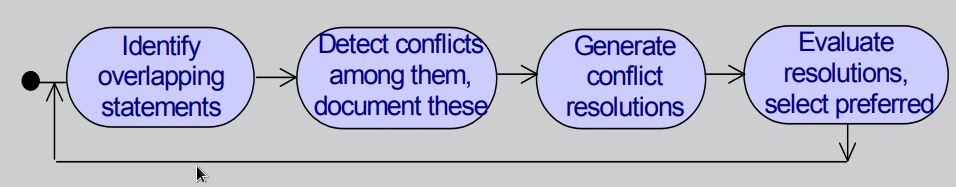
\includegraphics[width=0.9\textwidth]{images/managing_conflicts.png}
    \caption{چهار قدم چرخشی مدیریت تضاد‌ها}
\end{figure}

مدیریت تضاد‌های ضعیف و قوی در ۴ قدم انجام می‌شود:

\begin{enumerate}
    \item \lr{Identify overlapping statements}: شناسایی عباراتی که با هم مشترک
    هستند و در مورد یک مفهوم مشترک صحبت می‌کنند. شباهت‌های می‌توانند فاعل، فعل و
    مفعول باشند. عملیاتی که در کنار یکدیگر دچار تضاد نمی‌شوند. \begin{enumerate}
        \item پدیده‌های باز و بسته شدن در‌های خطار مفاهیم رایج در سبد
        نیازمندی‌های آن است.
        \item پدیده‌های بدست آوردن کتاب، قرض گرفتن و بازگرداندن کتاب نیز از
        مفاهیم رایج مرتبط به \lr{Book copy} می‌باشد.
    \end{enumerate}
    \item \lr{Detect conflicts among them, document these}: از میان جملات
    جمع‌آوری شده باید بررسی کنیم که ببینیم چه نظراتی با هم همپوشانی دارند. اگر
    از میان همپوشانی‌ها تضادی پیدا شد بایستی تضاد‌ها را داکیومنت کنیم. راه‌های
    تشخیص تضاد: \begin{enumerate}
        \item \lr{Informally} یا غیررسمی: به صورت غیررسمی اعلام می‌کنیم که
        همپوشانی عبارات با هم رضایت بخش هستند و تحت چه شرایطی راضی کننده نیستند؟
        به گونه‌ای که به صورت چشمی منطقی نیستند.
        \item استفاده از روش‌های اکتشافی یا \lr{Heuristics} (استفاده از درخت):
        براساس یک جدول مشخص می‌کند که جملات چگونه می‌توانند با یکدیگر تضاد داشته
        باشند.
        \item استفاده از روش رسمی یا \lr{Formally}: تکنیک‌های اثبات قضیه. در
        حالت رسمی نرم‌افزار‌های بحرانی را نمی‌توان \lr{UML} کرد چرا که نیاز به
        اثبات دارند. نمایش و اعتبارسنجی هم با استفاده از زبان‌های رسمی امکان
        پذیر می‌باشد.
        \item استفاده از الگو‌های تضاد که نسخه‌ای سبک‌تر از تکنیک‌های رسمی
        هستند. نتیجه به صورت گرافیکال می‌باشد.
    \end{enumerate}
    \item \lr{Generate conflict resolutions}: رزولوشن یک مفهوم است که کتاب مرجع
    برای مدیریت تضاد از آن استفاده می‌کند. هر  راه‌حلی که به ذهن مهندس نیازمندی
    رسید باید کامل آن را بیان کند.
    \item \lr{Evaluate resolutions, select preferred}: باید یکی از راه‌حل‌هایی
    که در مرحله پیشین ارزیابی کردیم را بررسی کنیم و بهترین آنها را انتخاب کنیم.
\end{enumerate}

\subsubsection*{نکات}

\begin{itemize}
    \item همانطور که می‌دانیم \lr{Statements} سبد ما می‌باشد و راه‌حل‌هایی که
    بدست می‌آوریم باید از جنس سبد باشد. اولین راه‌حل \lr{Drop} کردن می‌باشد.
    همچنین از دیگر راه‌حل‌های تغییر جمله و سازگار کردن آن است، حتی ما می‌توانیم
    برای حل تضاد جمله به آن جمله‌ای مناسب را اضافه کنیم.
    \item مهندس نیازمندی باید در \lr{Intra-viewpoint}ها بازه را تعیین کند.
    \item برای رفع تضاد ممکن است جمله‌ای را حذف، اضافه یا حتی تغییر دهیم. در این
    حین ممکن است بازم ایجاد تضاد صورت گیرد به همین خاطر ۴ قدم مدیریت تضاد‌ها به
    صورت چرخشی می‌باشد.
    \item ما باید عواملی که با هم تضاد دارند را بشناسیم که بتوانیم آن‌ها را
    مدیریت کنیم.
    \item باید بدانیم که کدام موارد باعث ایجاد تضاد می‌شوند و بعد از تغییر سبد
    می‌توانند دردسرزا شوند.
    \item معمولاً \lr{Conflict}خیز‌ها معمولاً در \lr{Overlap}های زیادی شرکت
    می‌کنند.
    \item جملاتی را باید استفاده کنیم که در \lr{Overlap}های زیادی شرکت داشتن و
    شرکتشان خوب و بدون تضاد بوده.
\end{itemize}

\subsection{تکنیک‌های داکیومنت کردن}

\begin{figure}[H]
    \centering
    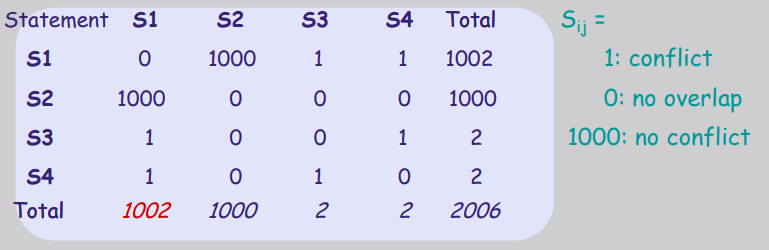
\includegraphics[width=0.9\textwidth]{images/systematic_process_table.png}
    \caption{تشخیص تضاد‌ها و همپوشانی‌ها}
\end{figure}

\subsubsection*{نکته}

\begin{itemize}
    \item باقی مانده نشان‌دهنده تضادهای بین دو جمله می‌باشد.
    \item خارج قسمت نشان‌دهنده همپوشانی مناسب و بدون تضاد است.
\end{itemize}

\begin{equation}
    Conflicts(S1) = remainderOf(1002/1000) \rightarrow 2
\end{equation}

\begin{equation}
    nonConflictingOverlaps(S1) = quotientOf(1002/1000) \rightarrow 1
\end{equation}

\begin{equation}
    Conflicts(Total) = remainderOf(2006/1000) \rightarrow 6
\end{equation}

\begin{equation}
    nonConflictOverlaps(Total) = quotientOf(2006/1000) \rightarrow 2
\end{equation}

\subsection{تکنیک‌های رفع تضاد}

برای رفع تضاد ۴ روش مطرح شده است که هر کدام از آن‌ها می‌توانند منجر به تولید
نیازمند‌های جدید شوند تا تضاد موجود در جمله را رفع کنند:

\subsubsection{خاص‌سازی منبع یا هدف تضاد}

تضاد در سطح جمله رخ می‌دهد، یعنی یک قانون به کل وارد می‌شود که یکسری جزئیات
دارد. نقض قانون بالایی به جز وارد می‌شود. هر کدام از جزئیات قوانین خودشان را
دارند و چون جز هم قانون خودش را دارد باعث ایجاد تضاد می‌شود. قانون جدید (جمله
جدید) در مورد کل سیستم نبوده و بلکه در مورد یک جز خاص می‌باشد. به جای اعمال
قانون به کل سیستم بایستی به یک نود و قشر مشخص این قانون جدید اعمال شود. معمولاً
در فاعل و مفعول رخ می‌دهد.

برای مثال:

\begin{itemize}
    \item به کاربران (\lr{Users}) اجازه داده شود که بتوانند از وضعیت کتابی که به
    امانت گرفته شده است مطلع شوند.
    \item دانشجویان نباید از وضعیت کتاب امانت گرفته شده مطلع باشند.
\end{itemize}

خاص‌سازی باید روی منبع یا رابطه کل به جز اعمال شود. در مثال بالا مشخص نیست که
کاربران دقیقاً چه قشری هستند و آیا شامل قشر دانشجویان می‌شود؟ پس بایستی قانونی
تعریف کنیم که مشخص شود چه گروهی قادر به مطلع شدن وضعیت باشند و چه گروهی
نمی‌توانند. به همین دلیل مجوز‌هایی برای \lr{Staff users} صادر می‌کنیم و مجوز
دیگری به نام \lr{Students}. در این دو گروه به روشنی می‌توان قابلیت‌هایشان را
شخصی‌سازی نمود. گروه خاص ما مفعول بوده است. چه کسانی بتوانند و چه کسانی نتوانند؟

\subsubsection{ضعیف‌تر کردن جملاتی که تضاد دارند}

در این روش معمولاً جمله سخت‌تر را ضعیف (\lr{Weak}) می‌کنیم. دقیقاً جزئی که قانون
را می‌بندد.

برای مثال:

\begin{itemize}
    \item پدر می‌گوید ساعت ۱۰ شب خانه باش اما مادر شما می‌گوید که هر چقدر بودی
    مشکلی نداره، در این جمله تضاد قوی را مشاهده خواهیم کرد.
    \item قرض گیرنده کتاب، باید کپی کتاب را سر مهلت سه هفته‌ای تحویل دهد مگر
    اینکه یک مجوز (\lr{Permision}) برای استفاده بیشتر کپی کتاب برای دانشجو صاد
    شود.
    \item مثال دقیق‌تر: دانشجو‌ها می‌توانند تا سه هفته کپی کتاب را از کتابخانه
    قرض بگیرند اما در صورتی که عضو انجمن علمی دانشگاه باشند می‌تواند ۵ هفته کتاب
    را داشته باشند.
\end{itemize}

\subsubsection{ری‌استور کردن}

در این روش تا زمانی که به تضاد بر نخورده‌ایم پیش می‌رویم و بعد از برخورد به تضاد
سیستم را به حالت قبل از تضاد خواهیم برد.

برای مثال دانشجو می‌خواهد کتاب را بیشتر از ۳ هفته قرض بگیرد، اما کتابخانه تنها ۳
هفته امکان قرض گرفتن را برای دانشجو فراهم کرده است. برای حل این تضاد کتابخانه از
ری‌استور کردن استفاده می‌کند و می‌گوید برای قرض گرفتن بیشتر از ۳ هفته، سر موعد
مهلت قرض گرفتن کتاب را تمدید کن.

\subsubsection{پرهیز از شرایط مرزی}

آخرین راه‌حل که سخت‌تر از بقیه می‌باشد این روش است که در مورد تضاد‌های ضعیف یا
(\lr{Weak conflict}) صادق خواهد بود. در این روش تلاش بر این است که شرایط مرزی را
برای تضاد‌ها به گونه‌ای کنترل کنیم که هیچ وقت رخ ندهند تا هدف سیستم را از بین
برود.

برای مثال، فرض کنید کتابخانه از یک کتاب مخصوص، تنها سه کپی دارد. اگر هر کدام از
این سه کپی را سه دانشجو مختلف قرض بگیرد، دانشجوی چهارم نمی‌تواند این کتاب را
درخواست کند. یعنی ریشه‌یابی یکسری کتاب که مرجع آن مشخص است که دیگر هیچ کپی از آن
در کتابخانه موجود نیست به این صورت رسماً رسالت کتابخانه زیر سوال رفته است. سوالی
که می‌تواند مطرح شود این است که آیا این نگرانی برای همه کتاب‌ها وجود دارد؟ باید
این مسئله بررسی گردد که برای چه کتاب‌هایی نیاز داریم شرط جدیدی را وضع کنیم. برای
کامل کردن مثال، فرض کنید از آن کتابی که در ابتدای فرضمان سه کپی داشتیم تنها دو
کپی قابل قرض دادن به دانشجو باشد و کپی آخر کتاب تنها زمانی قابل استفاده است که
خواننده کتاب درون کتابخانه باشد و نخواهد آن را به بیرون از کتابخانه ببرد.

برای مثال بالا ممکن است به دنبال الگوریتم‌های دسته‌بندی برویم که بتوانیم رضایت
را برای همه طرفین برقرار کنیم تا همه بتوانند از تمام کپی‌ها به صورت مناسب
استفاده کنند.

در شرایط مثال بالا سیستم کتابخانه بسیار اساسی‌تر خواهد شد و باید در صفات کلاس
مربوطه و نیازمندی‌ها خود اعلام کنیم که چند کپی از کتاب‌ها قابل قرض و چند کپی
قابل استفاده در محل کتابخانه می‌باشد.

\subsection{تمرین اول}

در یک سیستم مانند اسنپ، مسافر می‌خواهد نزدیک‌ترین ماشین به او تخصیص داده شود،
مدیر سیستم می‌خواهد در راستای طرح تشویقی خود رانندگانی با امتیاز بالاتر را به
مشتری تخصیص دهد. آیا تضادی می‌بینید؟ اگر بله از چه نوعی است و راه‌حل آن چیست؟

بله تضاد دارند، دو جمله وجود دارد:

\begin{itemize}
    \item کاربر به دنبال نزدیک‌ترین راننده اسنپ می‌باشد
    \item مدیر می‌خواهد راننده‌ای انتخاب شود که بالاترین امتیاز را داشته باشد.
    \item تضاد در جایی رخ می‌دهد که ممکن است راننده‌ای با امتیاز بالا در شعاع
    دورتری قرار داشته باشد.
    \item در این سناریو مشکلی برای راننده، مدیر و کاربر پیش نمی‌آید. پس تضاد
    ضعیف است. ما می‌توانیم با رویکرد \lr{Restore} کردن این تضاد را به گونه‌ای
    پوشش دهیم که همه راضی باشند.
    \item لزوماً امتیاز راننده می‌تواند ۵ ستاره اولین شعاع نزدیک به کاربر نباشد
    براساس درخواست کاربر مشخص می‌شود که کدام راننده با امتیاز بالا بایستی فیلتر
    شود و از بین آنها کدام راننده می‌خواهد درخواست کاربر را بپذیرد. این بدان
    معناست که درخواست کاربر برای رانندگانی که در همان شعاع هستند که امتیاز آن‌ها
    کم باشد، ارسال نمی‌شود.
\end{itemize}

\newpage

\subsection{مدیریت ریسک}

معمولاً در فاز‌های اولیه یک پروژه نرم‌افزاری، مهندسان نیازمندی و ذینفعان
انتظارات عجیبی را دارند:

\begin{itemize}
    \item محیط و نرم‌افزار همانگونه که انتظار دارند رفتار کند.
    \item برنامه توسعه نرم‌افزاری پروژه هماگونه که برنامه‌ریزی شده است رو به جلو
    باشد.
\end{itemize}

اما در حقیقت جا به جایی از \lr{System-as-is} به \lr{Sysmte-to-be} ممکن است دچار
ریسک‌های مختلفی شود.

\subsubsection{شدت ریسک یا \lr{Severity}}

درجه از دست دادن رضایت نسبت به یک هدف را شدت ریسک یا \lr{Severity} می‌گویند.

ریسک‌ها نقض (\lr{Not}) یک نیاز می‌باشند. وقتی یک نیاز به درستی انجام نشود یا به
هر دلیلی دیر انجام شود و نقض یک جمله باشد می‌توان گفت که به ریسک تبدیل شده است.
نکته حائز اهمیت آن است که ریسک روی یک جمله می‌باشد و روی دو جمله مانند تضاد‌ها
تاثیر ندارد.

ریسک‌ها به دو دسته تقسیم می‌شوند:

\begin{enumerate}
    \item مرتبط با محصول یا \lr{Product-related}
    \item مرتبط با فرایند یا \lr{Process-related}
\end{enumerate}

\subsubsection{مرتبط با محصول یا \lr{Product-related}}

بیشترین ارتباط را به مهندس نیازمندی دارد. الزاماتی که در طراحی یک سیستم بایستی
در نظر گرفته شود تا بتوانیم سیستم را در برابر آن‌ها تجهیز کنیم؛ لذا افرادی در
حوزه مدیریت ریسک کار می‌کنند که متخصص آن دامنه و سیستم هستند. یعنی کاملاً در
مورد دامنه تجربه و اطلاعات مناسب را دارا هستند. این افراد معمولاً جایگاه‌های
ثابتی در دامنه خود داشتند. مانند سیستم‌های حسابداری بانکی، سیستم‌های \lr{CRM} و
غیره. تمام حالات سیستم را دیده‌اند و در استراتژی‌های مختلف در برابر ریسک‌های
مرتبط را تجربه کرده‌اند. به عبارتی ساده‌تر یعنی به طور کل این افراد شناخت بسیار
کاملی نسبت به آن دامنه دارند.

این ریسک‌ها می‌توانند مانند مثال‌های زیر باشند:

\begin{itemize}
    \item ریسک در برابر ارسال و دریافت اطلاعات داخل برنامه‌ای؛ پیامی که ارسال
    می‌شود و قرار است به یک نفر برسد ریسک موارد زیر را دارد: \begin{itemize}
        \item پیام برای آن شخص مشخص ارسال نشود و به تمام کاربران داخل شبکه بدون
        اجازه ارسال شود. (\lr{Broadcastly send})
        \item پیام با تاخیر در شبکه ارسال شود و به دست دریافت کننده پیام برسد.
        \item شبکه شنود شود و محتوای پیام را بتوان به صورت غیرقانونی در شبکه
        مشاهده نمود.
        \item پیام قابلیت ویرایش پس از ارسال را داشته باشد.
    \end{itemize}
    \item سیستم حاوی احراز هویت می‌باشد و ریسک آن: \begin{itemize}
        \item اگر کاربر گذرواژه خود را فراموش کرده باشد؟ پس بایستی استراتژی
        مناسب در برابر این ریسک را در نظر بگیریم و برای این سیستم احراز هویت
        گزینه فراموشی گذرواژه را طراحی کنیم.
    \end{itemize}
\end{itemize}

\subsubsection{مرتبط با فرایند یا \lr{Process-related}}

تمام اتفاقاتی که در ارتباط مستقیم با محصول نمی‌باشد را شامل می‌شود. برای مثال
ممکن است ارزش پولمان کم‌تر شود یا یکی از اعضا/پرسنل‌مان استعفا دهد.اینگونه
ریسک‌ها مرتبط با مدیر پروژه می‌باشد.

\subsection{چرخه مدیریت ریسک}

\begin{itemize}
    \item فرایند پیدا کردن ریسک در پروژه‌های نرم‌افزاری یک فرایند تکرارپذیر
    می‌باشد که شامل سه مرحله‌ زیر می‌باشد: \begin{enumerate}
    \item \lr{Risk identification}: شناسایی ریسک: دقیقاً ریسکی در سیستم به صورت
    مشخص رخ می‌دهد؟ یا اتفاق افتاده است؟
    \item \lr{Risk assessment}: ارزیابی ریسک: آیا عواقب احتمالی بدی دارد؟
    می‌توان از آن جلوگیری کرد؟ آیا می‌توان تاثیرات رخدادش را مدیریت و کنترل کرد؟
    \item \lr{Risk control}: کنترل ریسک: مدیریت و کنترل ریسک به عنوان نیازمندی
    جدید
\end{enumerate}
    \item در این میان نکته بسیار مهم آن است که در چرخه تکرار بررسی ریسک ممکن است
    هر عملیات و اقداماتی منجر به ایجاد ریسک جدیدی شود.
    \item مدیریت ضعیف ریسک‌ها عامل اصلی شکست در پروژه‌های نرم‌افزاری می‌باشد.
    \begin{enumerate}
        \item اشتباه فکر کردن به جریانات پروژه که انگار قرار نیست هیچ فرایندی
        مشکل داشته باشد.
        \item عدم شناسایی و دستکم گرفتن ریسک‌ها که باعث ناقص و ناکافی در نظر
        گرفتن نیازمندی‌ها در پروژه شود.
    \end{enumerate}
\end{itemize}


\subsection{شناسایی ریسک}

در این قسمت به چهار تکنیک شناسایی ریسک در پروژه‌های نرم‌افزاری می‌پردازیم:

\subsubsection{چک لیست‌های ریسک}

بررسی چک لیست‌های ریسک هم می‌تواند در مورد ریسک‌های محصول باشد و هم در مورد
فرایند‌ها. برای مثال حوزه مالی اولین حوزه‌ای نیست که قبلاً وجود نداشته باشد و
دقیقاً این اولین سیستمی باشد که از قابلیت‌های مالی استفاده می‌کند. در حقیقت این
حوزه از قبل چندین بار مورد استفاده قرار گرفته شده است و توسط متخصصان مختلفی مورد
آزمون و تلاش بسیاری بوده که توانسته به بیشتر چالش‌ها و ریسک‌های آن پاسخ دهند. به
این ترتیب می‌توانیم تمام ریسک‌های آن را از قبل تهیه کنیم و بتوانیم در سیستم خود
آن‌ها را بررسی کنیم که اگر برخی قابلیت‌ها منجر به تولید ریسک شد بتوانیم راهکاری
برای آن طراحی و پیاده‌سازی کنیم. در حقیقت یک لیست راهنما از پیش تعیین شده
می‌باشد.

برای سناریو زیر می‌توان تمام ریسک‌ها را از قبل پیشبینی کرد و لیستی از باید‌ها را
برای آن به شکل زیر بررسی می‌کنیم:

وقتی ارسال کننده پیام بخواهد پیامی را برای دریافت کننده‌ای ارسال کند ریسک‌های
احتمالی موارد زیر خواهد بود:

\begin{itemize}
    \item درگاه پیام تغییر کند: استفاده از رویکردی امن.
    \item پیام در شبکه شنود شود: رمزنگاری و استفاده از شبکه‌های توزیع شده.
    \item تاخیر در ارسال پیام: بررسی زیرساخت‌های شبکه‌ای و حتی الگوریتم‌های
    ارسال و دریافت پیام.
\end{itemize}

نکته: محصولات همگی مشخص هستند و فرایند‌های آن‌ها کاملاً عمومیت دارد.

\subsubsection{بازبینی مولفه‌ها}

مولفه‌ها مخصوص محصول می‌باشد؛ المان‌ها در حقیقت همان مولفه‌ها هستند. آدم‌ها،
نرم‌افزار‌های موجود و نرم‌افزار‌هایی که قرار است توسعه داده شود، تماماً المان
محسوب می‌شوند. برای مثال در سیستم قطار المان سرعت‌سنج را مورد بررسی قرار می‌دهیم
تا ریسک‌هایش را متوجه شویم:

\begin{itemize}
    \item آیا می‌تواند وظیفه‌اش را به درستی انجام ندهد؟ بله ممکن است. وظیفه‌ آن
    بررسی حرکت قطار و سرعت آن است. عوامل مختلفی وجود دارد که می‌تواند سبب درست
    کار نکردن و یا توقف کار کردن آن شود.
    \item اگر سرعت فیزیکی قطار با سرعت اندازه‌گیری شده برابر نباشد یعنی این
    دستگاه مشکلی دارد.
    \item یکی از ریسک‌ها آن است که در حین حرکت یکی از مسافر‌ها اقدام به خراب کرد
    دستگاه کند.
\end{itemize}

یا مثال اپلیکیشن‌های وب و موبایل:

\begin{itemize}
    \item اگر کاربر به اشتباه دستش روی گزینه پاک کردن بخورد جا به جا مورد انتخاب
    شده حذف شود یک ریسک در نظر گرفته می‌شود.
    \item برای این ریسک طراحی دیالوگ را می‌توان در نظر گرفت که از او تایید مجدد
    برای انجام کار خودش گرفته شود.
    \item همچنین بعد از طراحی و پیاده‌سازی دیالوگ می‌توانیم در مورد قابلیت
    پیاده‌سازی لیست موارد پاک شده بپردازیم؛ یعنی سیستم را به گونه‌ای بنویسیم که
    قابلیت حذف آن به صورت \lr{Soft delete} باشد.
\end{itemize}

همه ریسک‌ها را نمی‌توان مدیریت کرد بلکه باید برخی از آنها پذیرفته شود. به همین
خاطر هر سیستمی بنا به مقدار آستانه تحمل خودش ریسک‌ها را می‌پذیرد. ریسک‌ها را
بررسی می‌کند اگر از مقدار آستانه کوچک‌تر بود مدیریتش را به کاربران می‌سپارد.
بارزترین مثال سیستم انتخاب واحد آموزشیار که به روشنی امکانات لود بالانس کردن
درخواست‌های کاربران زیاد را با پایین‌ترین کیفیت می‌تواند مدیریت کند. به خاطر
اینکه به کل سیستم صدمه‌ای وارد نمی‌کند، طراح سیستم از مدیریت این ریسک صرف‌نظر
می‌کند.

تمام عواقب \lr{Consequence} یک ریسک بایستی برآورد و بررسی شود. اگر نتوانیم یک
ریسک را مدیریت کنیم پس ممکن است رخ دهد. بعد از رخ دادن آن باید عواقب و تاثیرات
\lr{Side effect}های آن را در نظر بگیریم که چقدر می‌تواند مضر باشد و به سیستم
صدمه وارد کند. نوشتن تمام عواقب یک ریسک می‌تواند در کاهش نارضایتی‌ها تاثیرگذار
باشد.

\subsubsection*{آیا سیستم‌ها و سازمان‌ها از یک آستانه تحمل یکسان و مشخصی استفاده
می‌کنند؟}

خیر؛ هر سازمانی تحت شرایط و پروتکل‌های خاص خودش کار می‌کند و هر کسی نمی‌تواند
طبق میل و اراده خودش عمل کند. یک سازمان بررسی می‌کند که این مقدار آستانه چقدر
ارزش دارد.

پرسیدن چهار سوال زیر برای بررسی مولفه‌های ریسک، بایستی مولفه‌های خیلی بزرگ را
کوچک کنیم تا بتوانیم به سادگی به پاسخ سوالات زیر برسیم:

\begin{enumerate}
    \item 
\end{enumerate}

\subsubsection{درخت ریسک}

\subsubsection{استفاده از تکنیک‌های جمع‌آوری داده}
